% id: 0133
% book: RPM 중3-2 수학 · 01 삼각비
% section: 중단원 마무리하기
% figure: crop:fig-0133.png
% answer: $3$
% answer_source: 답지
% variant_level: 0 (원본 전사)
% 이 파일은 build.mjs 가 items.json 에서 만든다. 고칠 때는 items.json 을 고친다.
\noindent\begin{minipage}[t]{0.58\linewidth}\vspace{0pt}\raggedright 오른쪽 그림의 직각삼각형~$\pt{ABC}$에서 점~$\pt{I}$는 내심이고 $\angle\pt{BIC}=105^\circ$일 때, $3\sin\pt{A}+\cos\pt{A}\times\tan\pt{B}$의 값을 구하시오.\end{minipage}\hfill\begin{minipage}[t]{0.4\linewidth}\vspace{0pt}\centering \setlength{\dmfigw}{58.3pt}\ifdim\dmfigw>\linewidth\setlength{\dmfigw}{\linewidth}\fi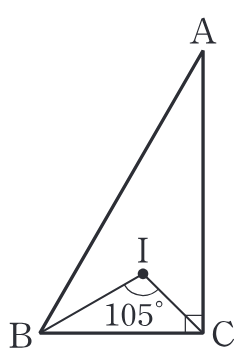
\includegraphics[width=\dmfigw]{figures/fig-0133.png}\end{minipage}\par
